\documentclass[12pt, a4paper]{ctexart}

% 页面设置
\usepackage{geometry}
\geometry{left=3cm, right=3cm, top=3cm, bottom=3cm}

% 常用宏包
\usepackage{graphicx}          % 插入图片
\usepackage{amsmath, amssymb}  % 数学公式
\usepackage{booktabs}          % 表格美化
\usepackage{hyperref}          % 超链接
\usepackage{titlesec}          % 自定义标题格式

% 增大行距
\linespread{1.15}  % 设置行距为1.5倍行距

% 设置英文字体与姓名一致
\renewcommand{\rmdefault}{ptm}  % 设置罗马字体为 Times New Roman,适用于所有英文部分

% 去除页眉页脚和页码
\pagestyle{empty}

% 自定义 \section 标题左对齐
\titleformat{\section}
  {\normalfont\Large\bfseries} % 格式:正常字体,大号,加粗
  {\thesection}{1em}{}         % 编号和间距

% 去除默认标题的居中对齐
\makeatletter
\def\maketitle{
  \begin{center} % 不要默认的居中
    \begin{flushleft} % 启用左对齐
    {\LARGE \textbf{\@title}}\\[1em] % 标题左对齐
    {\large \@author}\\[1em] % 作者左对齐
    \end{flushleft}
  \end{center}
}
\makeatother

% 题目信息
\title{Implimentation of Francis QR Algorithm \\ for Real Matrices}
\author{Haoyang Chen, School of Data Science, Fudan University 
    \\ 23307130004@m.fudan.edu.cn}
\date{} % 设置为空,以移除日期

\usepackage[ruled]{algorithm2e}                  %style 1
%\usepackage[ruled,vlined]{algorithm2e}          %style 2
%\usepackage[linesnumbered,boxed]{algorithm2e}   %style 3

\begin{document}

% 标题
\maketitle

% 正文部分
\section{Algorithm}

给定一个实矩阵 \( A \), 首先通过 Householder 镜像变换将其转换为上 Hessenberg 形式;
然后, 通过双重步位移隐式 QR 迭代将其转换为实 Schur 形式.
具体而言, 我们选择右下角 $2 \times 2$ 的子矩阵, 位移值通过子矩阵的特征值来确定, 为了避免可能的复数运算, 算法隐式地进行 QR 迭代;
QR 迭代的过程中, 算法通过小规模的 Householder 镜像变换, 处理 ``bulge''.
一次迭代后, 从下副对角线的右下角向左上角检索收敛为零的元素, 将其置零,否则继续迭代.
每次检索到一个收敛为零的元素, 算法都会使得矩阵的规模减小, 递归到更小的子矩阵上执行 QR 迭代.
最终, 算法递归至 $2 \times 2$ 的子矩阵, 迭代结束.
通过双重步位移 QR 算法, 得到的矩阵 $T$ 是拟上三角阵, 正交矩阵 $Q$ 记录相似变换, 算法还会输出迭代次数和运行时间, 其主要结构如下所述.
\\

\begin{algorithm}[H]
    \caption{Hessenberg Transformation}
    \KwIn{Square matrix $A$ of size $n \times n$}
    \KwOut{Hessenberg matrix $H$, orthogonal matrix $Q$ such that $Q^\top A Q = H$}
    $H = A$ \\
    $Q = \text{I}_n$ \\

    \For{$k = 0$ \KwTo $n-3$}{
        $x = A[k+1:n, k]$ \\
        $H = \text{house}(x)$ \\

        $A[k+1:n, k:n] = H \cdot A[k+1:n, k:n]$ \\
        $A[0:n, k+1:n] = A[0:n, k+1:n] \cdot H$ \\
        $Q[k+1:n, :] = H \cdot Q[k+1:n, :]$
    }

    \Return{$H, Q$}
\end{algorithm}

\par

算法利用 Householder 镜像变换将矩阵转换为上 Hessenberg 形式.
\\
\par

\begin{algorithm}[H]
    \caption{Francis Double Shift QR Algorithm for Hessenberg Matrices}
    \KwIn{Hessenberg matrix $H$, accumulation matrix $Q$, iteration index $i$}
    \KwOut{Updated Hessenberg matrix $H$, updated $Q$ such that $Q^\top \ Origin \ H \ Q = Updated \ H$}

    $n = i$, $m = n - 1$ \\
    $s = H[m-1, m-1] + H[n-1, n-1]$ \\
    $t = H[m-1, m-1] \cdot H[n-1, n-1] - H[m-1, n-1] \cdot H[n-1, m-1]$ \\
    $x = H[0, 0] \cdot H[0, 0] + H[0, 1] \cdot H[1, 0] - s \cdot H[0, 0] + t$ \\
    $y = H[1, 0] \cdot (H[0, 0] + H[1, 1] - s)$, $z = H[1, 0] \cdot H[2, 1]$ \\
    
    \For{$k = 0$ \KwTo $n-3$}{
        $House = \text{house}(\text{np.array}([x, y, z]))$ \\
        $H[k:k+3, :] = House \cdot H[k:k+3, :]$ \\
        $H[:, k:k+3] = H[:, k:k+3] \cdot House$ \\
        $Q[k:k+3, :] = House \cdot Q[k:k+3, :]$ \\
        update $x, y, z$ \\
    }
    $House = \text{house}(\text{np.array}([x, y]))$ \\
    $H[n-2:n, n-3:] = House \cdot H[n-2:n, n-3:]$ \\
    $H[:, n-2:n] = H[:, n-2:n] \cdot House$ \\
    $Q[n-2:n, :] = House \cdot Q[n-2:n, :]$ \\
    \Return{$H, Q$}
\end{algorithm}

\par

算法如此隐式地进行 QR 迭代, 并处理 "bulge".
\\
\par

\begin{algorithm}[H]
    \caption{Hessenberg to Schur Form}
    \KwIn{Hessenberg matrix $H$}
    \KwOut{Real Schur form $T$, orthogonal matrix $Q$ such that $Q^\top H Q = T$}
    $T = H$, $Q = \text{I}_n$, $m = dimension$, $\text{iteration\_time} = 0$ \\
    \lIf{$m \leq 2$}{trivial return}
    \While{$m > 2$}{
        $\text{found\_block} = \text{False}$ \\
        \For{$i = m-1$ \KwTo $0$ \textbf{step} $-1$}{
            \If{$|T[i, i-1]| < \text{tol} \cdot (|T[i-1, i-1]| + |T[i, i]|)$}{
                $T[i, i-1] = 0$, $m = i$, $\text{found\_block} = \text{True}$ \\
                \textbf{break}
            }
        }
        \lIf{\textbf{not} $\text{found\_block}$}{$T, Q = \text{(Algorithm 2)francis\_one}(T, Q, m)$}
        $\text{iteration\_time} = \text{iteration\_time} + 1$
    }
    \Return{$T, Q, \text{iteration\_time}$}
\end{algorithm}

\par

算法不断迭代, 直至矩阵规模减小至 $2 \times 2$,迭代结束. 

\par

\section{Code Structure}

\subsection*{Francis QR Double Shift Part 01: Calculation Function}
This section includes the core calculation functions used for Hessenberg transformation, Francis double-shift QR iteration, and Schur form computation.

\begin{enumerate}
    \item \textbf{house(x)}:
    \begin{itemize}
        \item \textbf{Input}: a vector \(x\) to be transformed.
        \item \textbf{Output}: a Householder transformation matrix \(H\) such that \(Hx = \|x\|e_1\), where \(e_1\) is the first standard basis vector.
        \item \textbf{Special Note}: Used to reflect vectors during Hessenberg and QR transformation.
    \end{itemize}

    \item \textbf{hessenberg(origin\_A)}:
    \begin{itemize}
        \item \textbf{Input}: a square matrix \(A\).
        \item \textbf{Output}: The Hessenberg form of \(A\) and the orthogonal transformation matrix \(Q\) such that \(Q^T A Q = H\).
    \end{itemize}

    \item \textbf{francis\_one(H, Q\_accum, i)}:
    \begin{itemize}
        \item \textbf{Input}: a Hessenberg matrix \(H\), the accumulated orthogonal matrix \(Q\_accum\), and the iteration index \(i\).
        \item \textbf{Output}: Updated Hessenberg matrix \(H\) and the accumulated orthogonal matrix \(Q\_accum\).
        \item \textbf{Special Note}: Performs a single iteration of the Francis double-shift QR algorithm.
    \end{itemize}

    \item \textbf{hessenberg\_to\_schur\_form(H, max\_iter=np.inf, tol=1e-16)}:
    \begin{itemize}
        \item \textbf{Input}: a Hessenberg matrix \(H\), maximum number of iterations, and tolerance for convergence.
        \item \textbf{Output}: Schur form \(H\), orthogonal transformation \(Q\_accum\), and the number of iterations performed.
    \end{itemize}

    \item \textbf{zeros\_hessenberg(H)}:
    \begin{itemize}
        \item \textbf{Input}: a Hessenberg matrix \(H\).
        \item \textbf{Output}: Hessenberg matrix with lower subdiagonal entries explicitly set to zero.
    \end{itemize}

    \item \textbf{generate\_test\_matrix(n, seed=None)}:
    \begin{itemize}
        \item \textbf{Input}: Matrix dimension \(n\) and an optional random seed.
        \item \textbf{Output}: a randomly generated square matrix of dimension \(n\).
    \end{itemize}

    \item \textbf{francis\_double\_shift\_qr(A)}:
    \begin{itemize}
        \item \textbf{Input}: a square matrix \(A\).
        \item \textbf{Output}: Schur form \(T\), orthogonal transformation matrix \(Q\), total iteration time, and execution time.
        \item \textbf{Special Note}: Combines Hessenberg transformation and Francis double-shift QR algorithm to compute the Schur form.
    \end{itemize}
\end{enumerate}

\subsection*{Francis QR Double Shift Part 02: Plot Figure Function}
This section includes functions for visualizing the performance metrics of the algorithm.

\begin{enumerate}
    \item \textbf{collect\_information(dimensions, seed=None)}:
    \begin{itemize}
        \item \textbf{Input}: a list of matrix dimensions and an optional random seed.
        \item \textbf{Output}: a dictionary of performance information, including orthogonality loss, forward error, and running time and so on.
    \end{itemize}

    \item \textbf{plot\_orthogonality\_loss(dimensions, orthogonality\_losses)}:

    \item \textbf{plot\_forward\_abs\_error(dimensions, forward\_abs\_errors)}:

    \item \textbf{plot\_forward\_rel\_error(dimensions, forward\_rel\_errors)}:
    
    \item \textbf{plot\_running\_time(dimensions, running\_times)}:
    
    \item \textbf{plot\_iteration\_time(dimensions, iteration\_times)}:
    
    \item \textbf{plot\_iterations\_per\_dimension(dimensions, iterations\_per\_dimension)}:
    
    \item \textbf{plot\_iterations\_per\_time(dimensions, iterations\_per\_time)}:
    
\end{enumerate}

\subsection*{Francis QR Double Shift Part 03: Demonstration}
This section demonstrates the use of the above functions for testing and visualizing the algorithm's performance.

\begin{enumerate}
    \item \textbf{one\_test(dimension)}:
    \begin{itemize}
        \item \textbf{Input}: Dimension of the square matrix to test.
        \item \textbf{Output}: Various metrics, including orthogonality loss, forward error, and eigenvalues, written to a text file.
    \end{itemize}

    \item \textbf{various\_test()}:
    \begin{itemize}
        \item \textbf{Input}: None (tests predefined dimensions).
        \item \textbf{Output}: Generates and saves performance plots for orthogonality loss, forward error, and iteration statistics.
    \end{itemize}
\end{enumerate}

\section{Numerical Experiments}


\subsection{Orthogonality Loss}

\begin{center}
    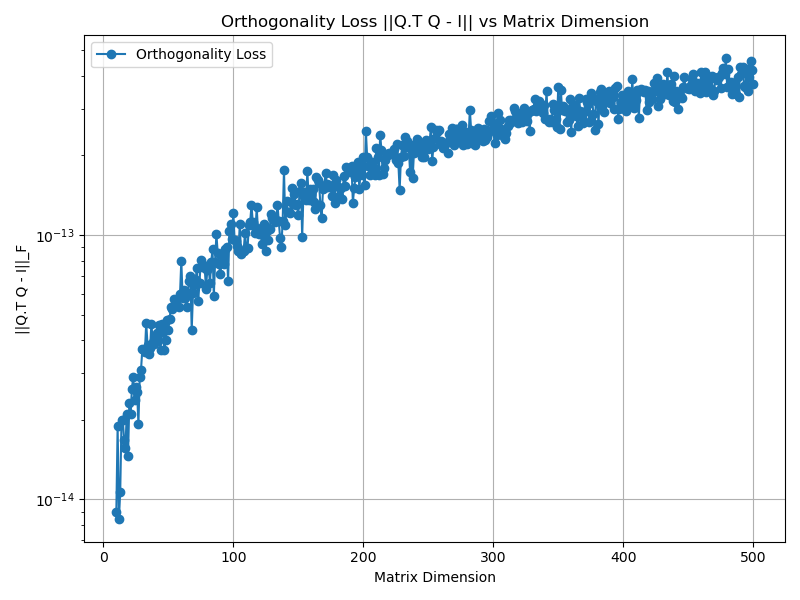
\includegraphics[scale=0.5]{orthogonality_loss.png}
\end{center}

\begin{center}
    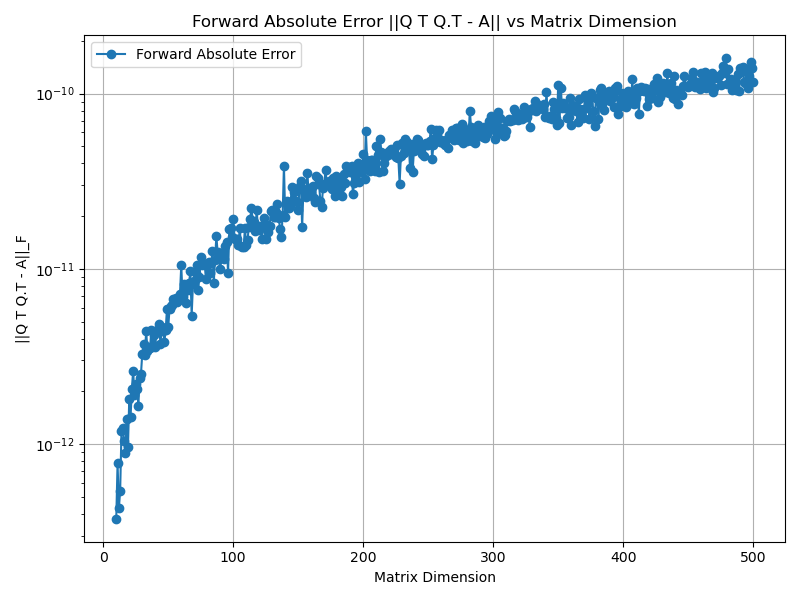
\includegraphics[scale=0.5]{forward_abs_error.png}
\end{center}

\begin{center}
    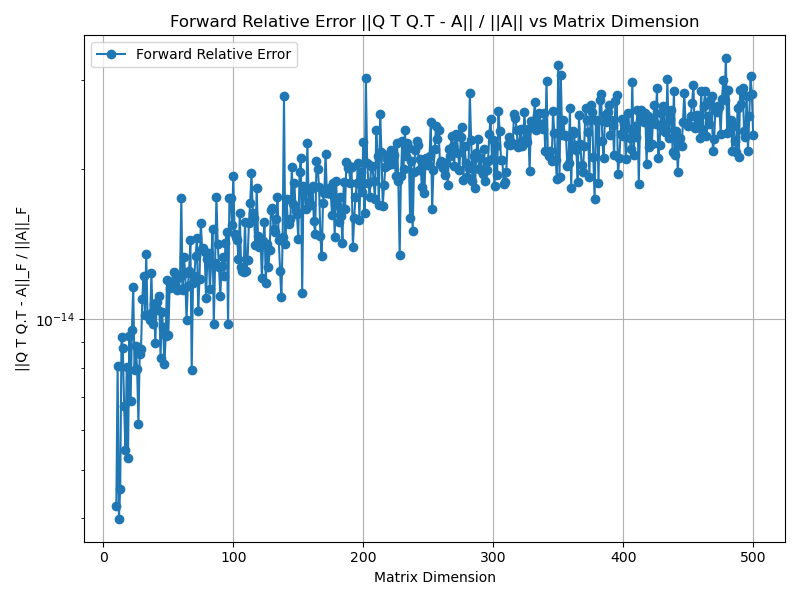
\includegraphics[scale=0.5]{forward_rel_error.png}
\end{center}

\subsection{Execution Time}

\begin{center}
    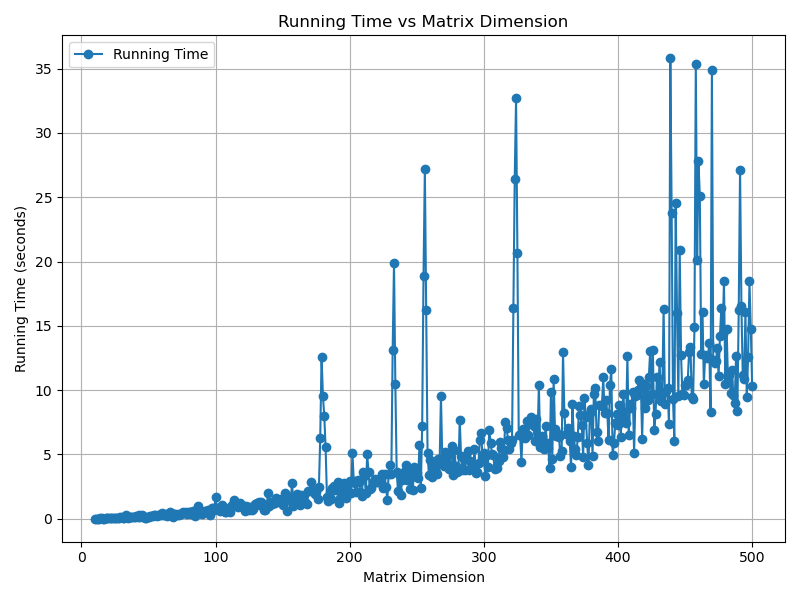
\includegraphics[scale=0.5]{running_time.png}
\end{center}

\subsection{Convergence Speed}

\begin{center}
    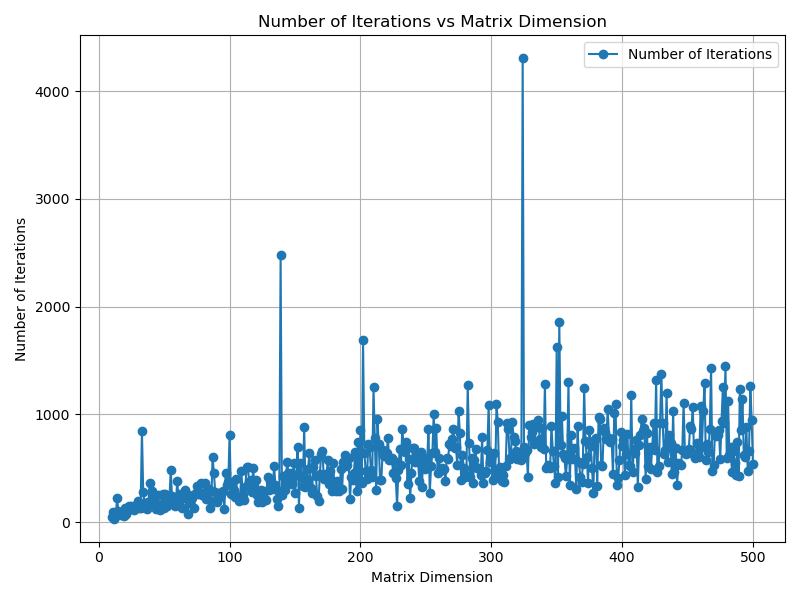
\includegraphics[scale=0.5]{iteration_time.png}
\end{center}

\begin{center}
    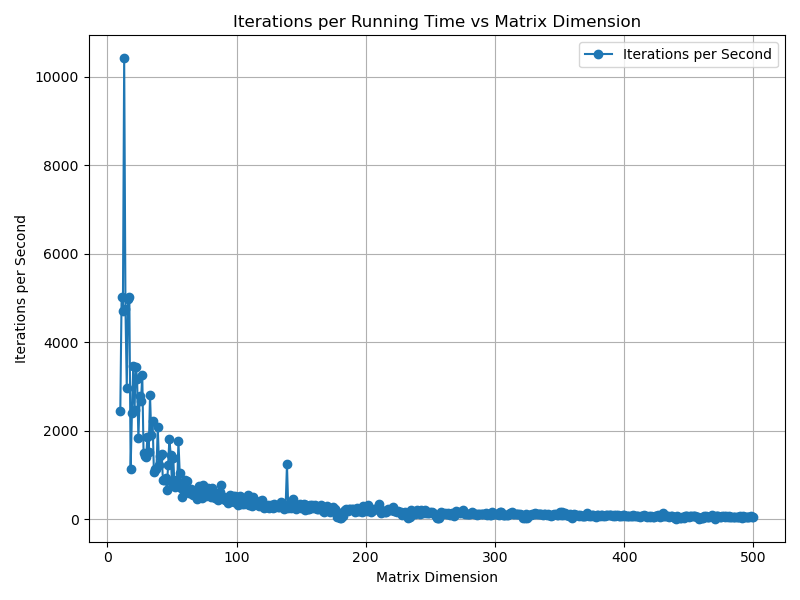
\includegraphics[scale=0.5]{iterations_per_time.png}
\end{center}


\section{Acknowledgements}

学生向授课教师邵美悦教授表达感谢, 感谢他在数值算法与案例分析课程中提供的指导和支持.
感谢本课程的助教们, 特别感谢助教叶爵达耐心批改我的作业, 提供反馈意见.
感谢舍友们在我探索路上的陪伴, 和他们的交流激励我不断进步.
\\
\\
\section{References}

[1] 徐树方, 高立, 张平文: 数值线性代数(第二版), 北京大学出版社2013年版.

[2] Lloyd N. Trefethen, David Bau III: 数值线性代数, 陆金甫, 关治译, 人民邮电出版社2006年版.

\end{document}
